\documentclass[12pt]{article}

\usepackage{a4wide}
\usepackage[utf8]{inputenc}
\usepackage[english]{babel}

\usepackage{amsmath}
\usepackage{biblatex}
\usepackage{courier}
\usepackage{csquotes}
\usepackage{enumerate}
\usepackage{graphicx}
\usepackage{hyperref}
\usepackage{listings}
\usepackage{svg}
\usepackage{color}

\definecolor{backcolour}{rgb}{0.95,0.95,0.92}

\lstdefinestyle{vcode}{
  backgroundcolor=\color{backcolour},
  basicstyle=\ttfamily\footnotesize,
  breaklines=true
}

\lstset{style=vcode}

\addbibresource{ref.bib}

\begin{document}

\title{Machine Learning Nanodegree: Capstone Project}
\author{Finbar Good}
\date{December 15, 2018}

\maketitle
   
\setlength{\parindent}{0cm}
\setlength{\parskip}{0.5\baselineskip}

\section{Definition}\label{i.-definition}

\subsection{Project Overview}\label{project-overview}
Since Google coined the term ``knowledge graph'', there has been an
increasing interest in the types of systems that fall under this broad
term\cite{ehrlinger2016towards}. Despite the interest - or perhaps
because of the lure of the name behind it - the term has been applied
widely and inconsistently. For the purposes of this proposal, we can
settle on this short definition: any store of facts represented as a
graph. And the sub-class of these graphs we are specifically interested
in are those that make use of the RDF standard.

RDF (Resource Description Framework) graphs \cite{w3RDF} represent facts
as a triple of IRIs or literal values. A triple consists of three parts:

\begin{itemize}
\item a subject: a thing or class, referred to using an IRI
\item a predicate: a property or relationship of the subject
\item an object: either the value subject's property, or the target of
  relationship
\end{itemize}

When the content of a graph is specified with RDF, the subjects and
objects form the nodes and the predicates form the edges. Because the
predicates are directed - going from subject to object - the graph is
directed.

\begin{figure}
  \centering
  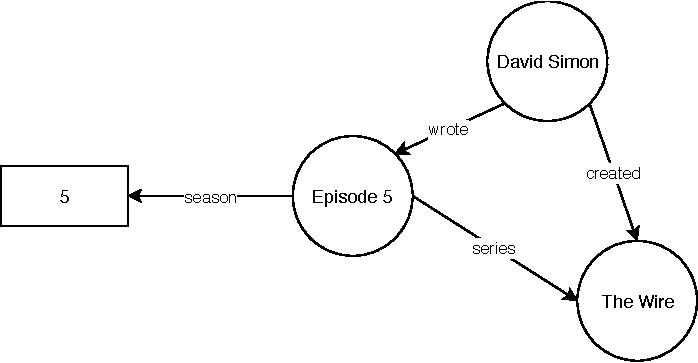
\includegraphics{images/rdf-the-wire.pdf}
  \caption{RDF example: some facts about The Wire}
\end{figure}

SPARQL is a query language designed for accessing RDF data, and was
elevated by the W3C to the recommended language for doing so
\cite{w3cSPARQL}. The following is an example of a very simple query in
SPARQL:

\begin{lstlisting}[language=SPARQL]
  SELECT ?creator
  WHERE { ?creator imbdo:created imdbr:the_wire }
\end{lstlisting}

In this example, we are looking for the entity (or entities) that
created another entity, imdbr:the\_wire. There are superficial
similarities with SQL, but they work in very distinct ways. What they
have in common is, from the point of view of a lay user, a steep
learning curve; only specialists tend to have the skills to create
queries in either language.

\subsection{Problem Statement}\label{problem-statement}
An area of research that has emerged in the past decade has been to
broaden the accessibility of knowledge graphs through parsing of natural
language queries (NLQ) to extract an answer from a knowledge graph (for
example \cite{Yahya:2012:NLQ:2390948.2390995}). Some of the more recent
efforts in the more general topic of question answering with a knowledge
base have looked at using neural networks to solve the problem (for
example \cite{liang2016neural}).

The challenge with accessing the data in knowledge graphs using RDF is
the query language, SPARQL. For many casual or non-technical users it is
an insurmountable barrier. To broaden the reach of such knowledge graphs
requires the automated translation of what casual users can produce,
natural language queries (NLQ), into something knowledge graphs can
parse, SPARQL.

This project aims to show that, at least in principal, a neural network
is a viable solution to automated translation of NLQs to SPARQL. Specifically:

\begin{enumerate}
  \item Download, merge, clean and split the LC-QuAD dataset (see \ref{data-exploration})
  \item Construct a word-oriented encoder-decoder neural network for training the translater
  \item Construct a SPARQL inference model that uses the trained encoder-decoder
  \item Train the encoder-decoder with the datasets
  \item Evaluate effectiveness of the inference model using the BLEU metric
  \item Repeat, altering hyper-parameters to investigate drivers of accuracy
\end{enumerate}

The models will be useful for considering the best approach to 
constructing a real, production-ready NLQ-to-SPARQL translater, supporting
search of a knowledge graph. Two key constraints are:
\begin{enumerate}
  \item Training datasets will, at least initially, be necessarily small
  \item The predicted SPARQL must be valid
\end{enumerate}

\subsection{Metrics}\label{metrics}

The BLEU score measures the degree of match between a generated sentence
and the reference sentence. This makes it useful to measure success of a
translation, in our case from natural language to SPARQL query. Values
range from 1 (perfect match) to 0 (perfect mismatch). Roughly, it is a
count of the number of distinct n-gram matches found in the reference
sentence, normalised by word count.

To use an example given in \cite{papineni2002bleu}, we have the
generated sentence:
  
\begin{lstlisting}[]
  It is a guide to action which ensures that the military always obeys the
  commands of the party
\end{lstlisting}

If we compare it to this reference sentence:

\begin{lstlisting}[]
  It is a guide to action that ensures that the military will forever heed
  Party commands
\end{lstlisting}

we see that 8 of the bigrams in the generated sentence are found in the
reference sentence. The bigram precision score is the number of matches
divided by the number of bigrams generated i.e.~8 / 17 = 0.47.

Shorter n-gram scores score precision, longer ones score fluency.

The actual calculation combines a precision measure with a penalty for 
the generated sentence being shorter than the reference sentence/s, the
brevity penalty. The brevity penalty is defined as:

\[ BP =
  \begin{cases}
    1               & \quad \text{if } c > r\\
    {\rm e}^{1-r/c} & \quad \text{if } c \leq r
  \end{cases}
\]

where c is the length of the candidate translation and r the reference
corpus length.

The BLEU score is then calculated as:

\[ BLEU = BP \cdot {\rm exp} \left( \sum_{n=1}^{N} w_n \log p_n \right) \]

where the weighted sum of n-gram precisions \(p_n\), up to \(N\), with weights \(w_n\).

I will use the BLEU metric to compare different training runs on the models.
As SPARQL queries are not ``fault tolerant'', we will need high scores for n
\textgreater{} 1.

\section{Analysis}\label{ii.-analysis}

\subsection{Data Exploration}\label{data-exploration}

The LC-QuAD dataset \cite{trivedi2017lc} was created
for the QALD (Question Answering over Linked Data) initiative
\cite{QALD}, a series of annual challenges to translate NLQ into SPARQL
(or the correct answer to the NLQ). The LC-QuAD dataset consists of 5000
questions and their corresponding SPARQL queries. The questions were
generated using the following workflow:

\begin{enumerate}
\def\labelenumi{\arabic{enumi}.}
\item
  Manually create query templates and a natural language equivalent
  template
\item
  Extract a list of entities
\item
  Manually create a whitelist of predicates
\item
  For each entity, extract subgraph centred on the entity from DBpedia,
  extending 2 hops away
\item
  Generate a query from each fact in these subgraphs, restricted to the
  predicate whitelist
\item
  The populated template is then mapped to the natural language
  equivalent
\item
  Humans review the final result, paraphrasing and/or correcting the
  results
\end{enumerate}

Here is an example entry from the dataset:

\begin{lstlisting}[]
  {
    "_id": "285", 
    "corrected_question": "In which state is the Channel district?", 
    "intermediary_question": "What is the <state> of Channel District ?", 
    "sparql_query": " SELECT DISTINCT ?uri WHERE { <http://dbpedia.org/resource/Channel_District> <http://dbpedia.org/ontology/state> ?uri } ", 
    "sparql_template_id": 2
  }
\end{lstlisting}

In this exercise, we are only interested in 2 fields:

\begin{itemize}
  \item 
    corrected\_question: the natural language question. We will normalise these, 
    making their case consistant, removing punctuation etc.
  \item
    sparql\_query: the target SPARQL query. This will consist of valid SPARQL statements,
    where each token is well-formed. The only exception is that grouping or continuation 
    symbols aren't forced to have space around them; we will enforce this so they are treated
    as separate tokens. Otherwise we will not perform any normalization.
\end{itemize}

\subsection{Exploratory Visualization}\label{exploratory-visualization}

\begin{figure}
  \centering
  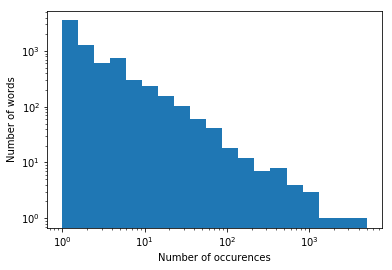
\includegraphics{images/question_word_distribution.png}
  \caption{Distribution of words in questions}
  \label{fig:question_word_distribution}
\end{figure}

\begin{figure}
  \centering
  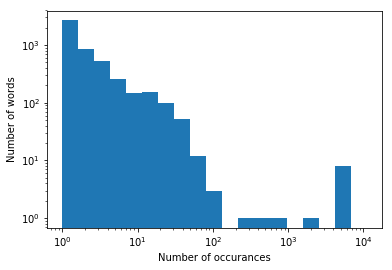
\includegraphics{images/query_word_distribution.png}
  \caption{Distribution of words in queries}
  \label{fig:query_word_distribution}
\end{figure}

The word distribution characteristics of the NLQs and SPARQL statements differ
in one significant respect: a small but significant number of SPARQL tokens
are very frequent.

The distribution for NLQs is shown in figure \ref{fig:question_word_distribution}.
We can see this follows the expected power law distribution.

The distribution for SPARQL is a little different (see figure \ref{fig:query_word_distribution}).
There are a significant number of tokens that are not distributed the same as the other
tokens. This was mentioned already above: SPARQL statements are a mixture of a small number
of keywords and a large number of identifiers of objects, predicates and literals, the things
and relations that the queries are about. 

The top 15 SPARQL tokens is given in table \ref{tbl:sparql_token_freq}. In addition to 
the SPARQL keywords and punctuation, we also see the predicate for type (high in 
frequncy as narrowing a query by type is so common) as well as a number of classes that
may be due to a skewing caused by the method for their generation.

\begin{table}
  \centering
  \begin{tabular}{ l | r }
    \textbf{Word} & \textbf{Count} \\
    \hline
    \texttt{?uri} & 11010 \\
    \texttt{.} & 6465 \\
    \texttt{WHERE} & 5000 \\
    \texttt{\{} & 5000 \\
    \texttt{\}} & 5000 \\
    \texttt{?x} & 4740 \\
    \texttt{SELECT} & 4632 \\
    \texttt{DISTINCT} & 4632 \\
    \texttt{<http://www.w3.org/1999/02/22-rdf-syntax-ns\#type>} & 1925 \\
    \texttt{COUNT(?uri)} & 658 \\
    \texttt{ASK} & 368 \\
    \texttt{<http://dbpedia.org/ontology/TelevisionShow>} & 236 \\
    \texttt{<http://dbpedia.org/ontology/Person>} & 132 \\
    \texttt{<http://dbpedia.org/ontology/Film>} & 113
  \end{tabular}
  \caption{Top 15 tokens by frequency in the SPARQL queries}
  \label{tbl:sparql_token_freq}
\end{table}

\subsection{Algorithms and Techniques}\label{algorithms-and-techniques}

The translation is done with a recurrent neural network (RNN), specifically an
encoder-decoder composed of Long Short Term Memory (LSTM) layers. These RNNs have 
been used to improve the "memory" of the network, so that the model can be
trained to pick up on the larger scale patterns required to translate sentences
of a dozen or more words.

I also add an embedding layer as it should improve the computational 
efficiency of the input questions and queries. However, as the network is being
trained to classify - that is to choose the best next token in the sequence -
we are required to one-hot encode the predicted query. 

The final decoder layer was a dense layer with softmax activation.

I then reused the trained network to generate queries from questions. The question
is fed to the encoder, whose LSTM state and a start token are passed to the decoder,
to predict the first token of the query. We loop this until the decoder predicts an
end token (or hits the maximum query length).

I explored the effects of varying the following:

\begin{itemize}
  \item Batch size (size of batch between back propagation), to see the effect of speed of learning
  \item Dropout, to see the degree to which we overfitting is a problem
  \item Number of neurons, to explore where the sweet spot for over/underfitting might lie
  \item Optimizer, to compare two that are recommended for LSTMs, Adam and rmsprop
\end{itemize}

The datasets are shuffled and split into training, validation and test sets.

The training and prediction were done on GPUs.

\subsection{Benchmark}\label{benchmark}

I used the model described in \cite{soru2018neural} as the
benchmark. It is also uses a neural network for end-to-end translation
of NLQs to SPARQL queries - but is obviously more complex and subjected
to many more refinements and iterations, possibly setting a rather
unrealistically high bar. Nonetheless it was the only comparable exercise 
I found that used the BLEU metric.

Depending on the refinement, they achieved BLEU scores between 80.89\%
and 99.29\%. Their dataset was generated directly from DBPedia.

\section{Methodology}\label{iii.-methodology}

\subsection{Data Preprocessing}\label{data-preprocessing}

The data was downloaded from the
\href{https://github.com/AskNowQA/LC-QuAD/}{GitHub pages of the LC-QuAD project}.
I then processed the data as follows:

\begin{itemize}
  \item 
    Consolidated the 2 files, their training and test datasets.
  \item 
    Loaded, parsed JSON into dict structure, and mapped the 
    "corrected\_question" and "sparql\_query" fields to separate variables.
  \item 
    The NLQs were cleaned by setting to lowercase and removing punctuation.
  \item 
    I ensured that the SPARQL queries were properly tokenized, ensuring spaces
    around grouping and continuation symbols.
  \item
    Two datasets were generated from the SPARQL queries: one set had a 
    start token pre-pended, to use as inputs to the decoder; the other
    had an end token append, to use as outputs.
  \item 
    All datasets were then tokenized.
\end{itemize}

\subsection{Implementation}\label{implementation}

Implementation was done with a Jupyter notebook, running on TPUs on Colaboratory.

Following the data pre-processing:

\begin{itemize}
  \item  
    Sets of hyper-parameters were generated, for (1) number of neurons
    [64, 128, 256] (2) batch size [32, 64] (3) optimizer ['adam', 'rmsprop'], 
    and (4) dropout [none, 50\%]
  \item
    For each set, an encoder-decoder model was instantiated, and trained on 
    the training set (split between training-validation-test was 81\%-9\%-10\%).
    The training was run for 100 epochs (based on observations of the divergence
    of training and validation loss, running for any longer wouldn't have been
    worth it). As this is a classification problem, I used the categorical crossentropy
    loss function. Although it is not as helpful as BLEU metric for gauging the 
    fluency of translation, I also tracked the accuracy metric.
  \item 
    A plot of the loss function for training and validation sets was produced at
    the end of the training run, mainly to gauge overfitting, the biggest problem
    with a relatively small dataset.
  \item 
    The training and test datasets were then run through evaluator, which would 
    generate predicted SPARQL queries for each NLQ in the datasets, and both
    dump the translations (for inspection) and calculate 1-to-4 gram, weighted
    BLEU scores.
\end{itemize}

As Colaboratory is a free platform with a time limit for use, the actual iterations
through the hyper-parameter sets had to be restarted manually. As a result, the 
BLEU metrics were consolidated in a selective fashion manually (only picking those
that showed the main drivers in improvement to the BLEU scores).

\subsection{Refinement}\label{refinement}

The main challenge that became apparent was the inability of the model
to generalize past the most common words, which were the SPARQL keywords
and punctuation, plus a few predicates and classes that occur in many
queries. You can see the signs of overfitting in figure \ref{fig:loss-metric-shows-overfitting}.

\begin{figure}
  \centering
  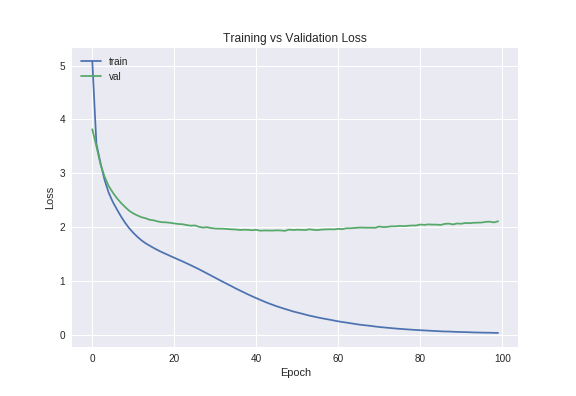
\includegraphics[width=12cm]{images/loss_model_256_100_64_adam_00_00.png}
  \caption{Overfitting evident in the loss function}
  \label{fig:loss-metric-shows-overfitting}
\end{figure}

I had already implemented a simple grid search of hyper-parameters from the start,
but I augmented this with the addition of dropout (leaving it out was an oversight).
This greatly improved the translations (although they remained far from useable,
as we will see). 

\section{Results}\label{iv.-results}

\subsection{Model Evaluation and Validation}\label{model-evaluation-and-validation}

\begin{figure}
  \centering
  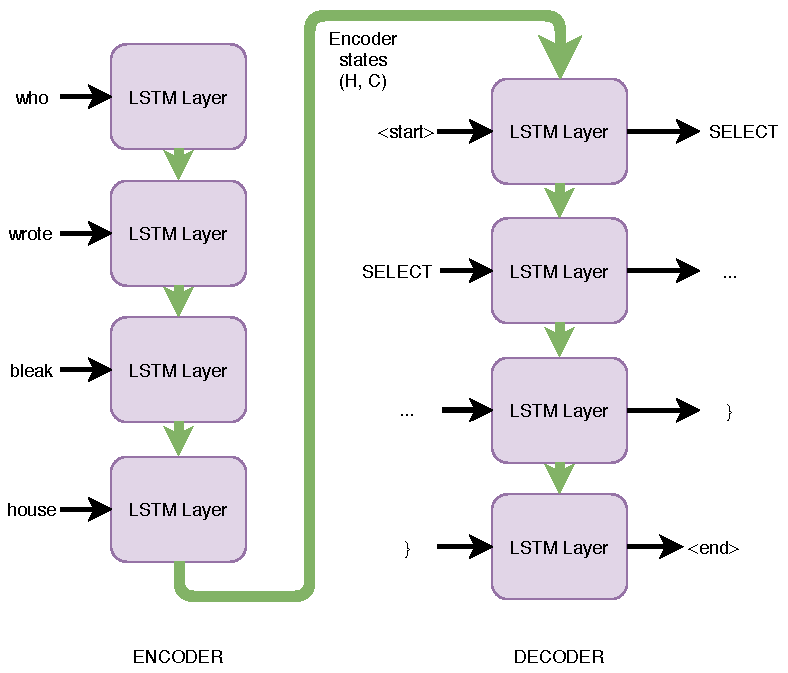
\includegraphics{images/encoder-decoder-training.pdf}
  \caption{Encoder-Decoder model used in training}
  \label{fig:encoder-decoder-training}
\end{figure}

\begin{figure}
  \centering
  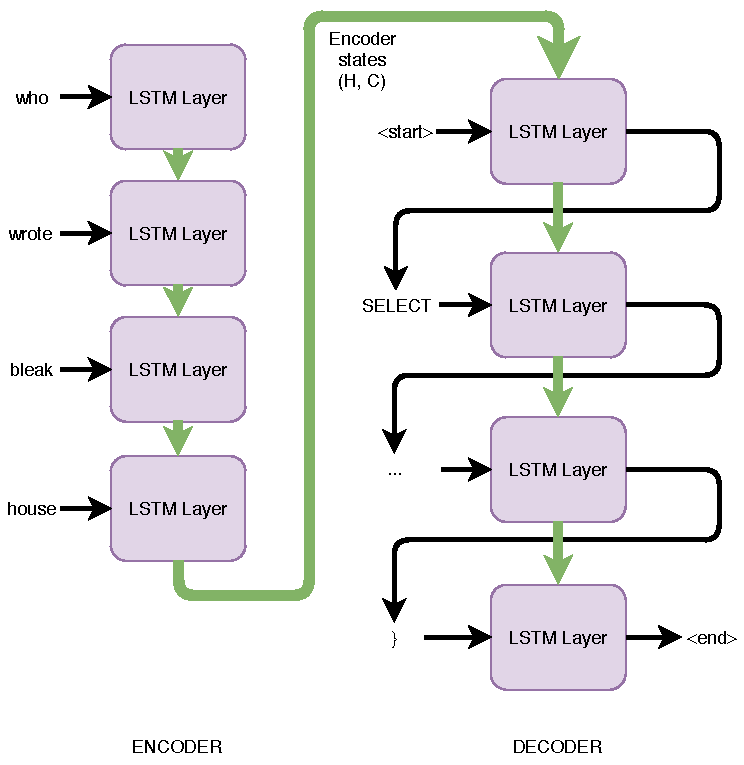
\includegraphics{images/encoder-decoder-translating.pdf}
  \caption{Re-use of the trained model to carry out translation}
  \label{fig:encoder-decoder-translating}
\end{figure}

Figures \ref{fig:encoder-decoder-training} and 
\ref{fig:encoder-decoder-translating} for high-level view of the final training
and translating models respectively.

The final model/s were the result of my attempt to port the ideas in 
a character-based translater described in 
\href{https://blog.keras.io/a-ten-minute-introduction-to-sequence-to-sequence-learning-in-keras.html}{a blog on the Keras site},
to a word-based version.

The model's selling point was that it was able to handle sequences of
arbitrary length, something necessary for the problem of arbitrary length
questions. Although the final translations themselves were disappointingly 
far from useable, the fact that after training on a relatively small 
dataset (for a neural network) they were able to start predicting some
of the features of a well formed query (for example, balanced parentheses),
was impressive, and a vindication of exploring end-to-end translation with
a neural network.

Using grid search and with BLEU metric as the measure, the following were 
the best hyper-parameters:

\begin{enumerate}
  \item neurons = 256 - lower neurons couldn't learn enough
  \item batch size = 64 - although very little variation with this
  \item optimiser = rmsprop - the difference with Adam was small
  \item dropout = 0.5 - this had the biggest effect
\end{enumerate}

The BLEU scores were robust to repeated runs (which used random shuffles
of the source dataset to compose training-validation-test). However,
the metric failed to flag runs where the training fell into a sub-optimal
minima: even with the above hyper-parameters, the training could fall
in on just predicting the most common tokens over and over, and do that
for \textit{all} input sentences.

\subsection{Justification}\label{justification}

\begin{figure}
  \centering
  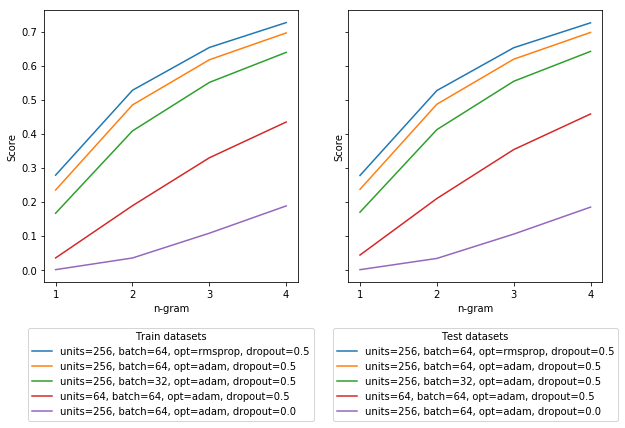
\includegraphics[width=14cm]{images/bleu_metrics.png}
  \caption{BLEU Metrics}
  \label{fig:bleu-metrics}
\end{figure}

A comparison of the BLEU scores is shown in figure \ref{fig:bleu-metrics}.
We see for the 4-gram BLEU score (evenly weighted) a value exceeding 70\%, 
which when taking in to account the simplicity of the model and the small
dataset, seems to compare well to the range of 80.89\%-99.28\% claimed in
\cite{soru2018neural}.

Our suspicions should be raised by the similarity between the scores
for the training and test sets. Inspection of the translations gives us
a clue as to the reason: the model is learning the common words found in
the SPARQL queries, and some structural aspects of those queries, but is
failing to learn the entities and predicates. The particular subsets of 
entities and predicates are what vary between any two randomly selected
sets; if the model is ignoring them, then it will perform equally well / 
badly on each of them.

To be of use, the end-to-end approach will need significant refinement in
the model, or improvement in the datasets to train on.

\section{Conclusion}\label{v.-conclusion}

\subsection{Free-Form Visualization}\label{free-form-visualization}

The following are a few sample translations that were produced, produced 
after the model had been trained with the best hyper-parameter set found:

\begin{lstlisting}[]

  Question: 
    what is the team name of st viator high school

  Target: 
    select distinct ?uri where {
      <http://dbpedia.org/resource/st._viator_high_school> <http://dbpedia.org/property/teamname> ?uri 
    }

  Predicted:
    select distinct ?uri where {
      ?uri <http://dbpedia.org/ontology/associatedband> <http://dbpedia.org/resource/foxy_brown_(rapper)>
    }

\end{lstlisting}

\begin{lstlisting}[]

  Question:
    how many universities are there whose country's capital is oslo

  Target:
    select distinct count(?uri) where {
      ?x <http://dbpedia.org/property/capital> <http://dbpedia.org/resource/oslo> .
      ?uri <http://dbpedia.org/ontology/country> ?x .
      ?uri <http://www.w3.org/1999/02/22-rdf-syntax-ns#type> <http://dbpedia.org/ontology/university>
    }

  Predicted:
    select distinct count(?uri) where {
      ?uri <http://dbpedia.org/property/team> <http://dbpedia.org/resource/chicago_bulls> . 
    }

\end{lstlisting}

You can see that it is predicting valid SPARQL statements, but throwing
in totally unrelated entities and predicates. For a given training run,
the entities and predicates would be drawn from a small set (usually 
frequently occurring in the corpus).

Here is an example from when one of the training runs went in the wrong direction:

\begin{lstlisting}[]

  Question:
    name the nearest city to lake victoria

  Target:
    select distinct ?uri where {
      <http://dbpedia.org/resource/lake_victoria> <http://dbpedia.org/ontology/nearestcity> ?uri
    }

  Predicted:
    select distinct ?uri where ?uri . }

\end{lstlisting}

It is not valid SPARQL, and only consists of keywords, punctuation, or a commonly
used variable name \(?uri\).

\subsection{Reflection}\label{reflection}

In summary, these were the project steps:

\begin{enumerate}
  \item 
    The broad area of interest - searching a knowledge graph - was selected
  \item 
    A problem narrow and specific enough in the area was defined (can a fluent
    search interface be created for an RDF graph)
  \item
    The largest, clean and freely accessible dataset pairing NLQs and SPARQL
    queries was found
  \item
    The datasets were inspected for their characteristics, and appropriate cleaning
    and tokenization was selected
  \item
    A survey of research in the area was done, looking for approaches that
    leveraged something in my machine learning experience e.g. neural networks
  \item
    A published, character-based, non-fixed length translater was adapted to
    work at the word-level, and constructed with Keras / Tensorflow
  \item 
    Different combinations of hyper-parameters were tested, suggesting the 
    optimal combination
  \item
    A SPARQL predicter was used to generate translations, enabling the BLEU 
    metric to examine fluency
\end{enumerate}

Construction of the translater was by far the most challenging aspect, and 
the time it consumed prevented me for developing the model further. I never
found a model implementation of a word-based encoder-decoder that was simple
enough as a starting point. Small things like not being aware of the zero\_mask
parameter cost many days of work!

It was a very useful experience in learning the limitations of neural networks,
but it also stimulated many ideas about it can be adapted to solve the problem
of search in knowledge graphs.

\subsection{Improvement}\label{improvement}
If you wished to pursue the end-to-end neural machine translation 
approach, you could consider the following to improve the performance:

\begin{enumerate}
  \item 
    Increase the dataset size by generating many times more questions
    with larger entity and predicate sets, and more SPARQL templates
  \item 
    Play with deep, LSTM layers (Google Translate reportedly uses networks that are 8 deep) 
    \cite{wu2016google}
  \item
    Add features like attention, to improve the "memory" of the network \cite{luong2015effective}
\end{enumerate}

Translating NLQ to SPARQL has a couple of essential requirements that 
probably don't apply as much to, say, french to english translations:

\begin{enumerate}
  \item It must generate valid SPARQL
  \item It must return results about the entities in their question
\end{enumerate}

A simple approach to try to guarantee this would be to break the 
translation down in to stages:

\begin{enumerate}
  \item 
    Entity extraction, so as to ensure these end up in the SPARQL query
  \item 
    Train a model to predict a specific SPARQL template from an NLQ, 
    and populate with the entities (and predicates) extracted
\end{enumerate}

This could be a rabbit hole, the kind that end-to-end NN translation
neatly sidesteps, but something only more experimentation will prove.

\printbibliography
   
\end{document}
